\chapter{Protocollo di somministrazione e scoring del Baby-FE}
\label{app:babyfe}

\thispagestyle{plain}

\noindent\textbf{CODICE:}~\rule{3.2cm}{0.4pt}\quad\textbf{ETA IN MESI:}~
ule{2.4cm}{0.4pt}\quad\textbf{DATA DI VALUTAZIONE:}~\rule{2.8cm}{0.4pt}

\clearpage
\noindent\centerline{%
\rotatebox{90}{%
\footnotesize
\setlength{\tabcolsep}{3pt}
\begin{tabular}{|p{3.2cm}|p{2.8cm}|p{7.8cm}|p{5.0cm}|p{1.0cm}|}
\toprule
  \textbf{ITEM e DOMINIO} & \textbf{MATERIALE} & \textbf{ISTRUZIONI} & \multicolumn{2}{|p{6.21cm}|}{\textbf{PUNTEGGI0}} \\
\midrule
  \textbf{1.LETTURA CONDIVISA} \newline \textbf{Dominio: }Attenzione & Libro cane & Posizionarsi a fianco del bambino. \newline Dare il libro in mano al b, lasciandolo esplorare per circa 1 minuto. \newline Poi dire: \textbf{\emph{``Guarda, adesso proviamo a leggere insieme il libro cane. Ascolta!''}} & \textbf{2}: b mantiene l'attenzione per l'intera durata della storia, rispettando il ritmo dell'adulto. \newline *ammesse lievi fluttuazioni attentive o brevi iniziative partecipative, purché pertinenti alle immagini o al contenuto del libro. \newline \textbf{\emph{1}}: attenzione discontinua per buona parte dell'attività o facilmente esauribile. \newline \textbf{\emph{0}}: b non sostiene l'attenzione durante l'attività o non riesce ad adattarsi al ritmo proposto dall'adulto. & \textbf{2} \newline \textbf{1} \newline \textbf{0} \\
  \multicolumn{5}{|p{20.64cm}|}{\textbf{NOTE:}} \\
\bottomrule
\end{tabular}
}}

\clearpage
\noindent\centerline{%
\rotatebox{90}{%
\footnotesize
\setlength{\tabcolsep}{3pt}
\begin{tabular}{|p{3.2cm}|p{2.8cm}|p{7.8cm}|p{5.0cm}|p{1.0cm}|}
\toprule
  \textbf{ITEM E DOMINIO} & \textbf{MATERIALE} & \textbf{ISTRUZIONI} & \multicolumn{2}{|p{6.21cm}|}{\textbf{PUNTEGGIO}} \\
\midrule
  \textbf{2.MEMORY} \newline \textbf{Dominio: }WM & \textbf{\uline{SERIE A}}\textbf{: }6 carte \newline (2 cane + 2 palla + 2 pesce) \newline \textbf{\uline{SERIE B}}\textbf{: }6 carte \newline (2 gatto + 2 casa + 2 topo) & \textbf{\uline{SERIE A}}\textbf{: }\textbf{\emph{``Guarda bene le carte }}\emph{(indicandole e nominandole in ordine):}\textbf{\emph{ il cane, la palla e il pesce. Ricordati dove sono perché adesso le nascondiamo! Dov'è il cane? E la palla? E il pesce?''}} \newline Posizionare le carte a distanza regolare, con una carta in posizione centrale rispetto al b e le altre due equidistanti ai lati destro e sinistro (cane alla mia destra) \newline \textbf{\uline{SERIE B}}\textbf{: }\textbf{\emph{``Adesso giochiamo con altre carte. Guarda bene le carte }}\emph{(indicandole e nominandole in ordine--- gatto alla mia destra)}\textbf{\emph{: il gatto, la casa e il topo. Ricordati dove sono perché adesso le nascondiamo! Dov'è il gatto? E la casa? E il topo?''}} \newline \textbf{NB }rigirare le carte una volta che b le indovina & \textbf{2}: 6/6 corrette \newline \textbf{1}: 4-5/6 corrette \newline \textbf{0: }3/6 corrette \newline *qualsiasi modalità di risposta è accettata (pointing, sguardo…) & \textbf{2} \newline \textbf{1} \newline \textbf{0} \\
  \multicolumn{5}{|p{20.64cm}|}{\textbf{NOTE:}} \\
\bottomrule
\end{tabular}
}}

\clearpage
\noindent\centerline{%
\rotatebox{90}{%
\footnotesize
\setlength{\tabcolsep}{3pt}
\begin{tabular}{|p{3.2cm}|p{2.8cm}|p{7.8cm}|p{5.0cm}|p{1.0cm}|}
\toprule
  \textbf{ITEM E DOMINIO} & \textbf{MATERIALE} & \textbf{ISTRUZIONI} & \multicolumn{2}{|p{6.21cm}|}{\textbf{PUNTEGGIO}} \\
\midrule
  \textbf{3.MEMORY CON} \newline \textbf{SPOSTAMENTO} & \textbf{Utilizzare la }\textbf{\uline{SERIE B }}\textbf{dell'item precedente: }6 carte (2 gatto+ 2 casa+ 2 topo) & \textbf{``}\textbf{\emph{Sei stato bravissimo. Ecco le carte che hai trovato…''. }}\emph{Mostrare nuovamente le carte al bambino, poi coprirle di nuovo. }\textbf{\emph{``Attenzione, adesso si muovono!''}} \newline \textbf{Step 1: }Girare le carte e spostare la carta 1 con la carta 2 partendo da sinistra ``\textbf{\emph{Dov'è la casa?''}} (= oggetto corrispondente alla posizione 1). Ricoprire poi le carte prima di procedere la richiesta 2. \newline \textbf{Step 2: }Scambiare la carta 2 con la carta 3 partendo da sinistra \textbf{\emph{``Dov'è il topo?}}  (=oggetto corrispondente alla posizione 3). \newline \textbf{\emph{``E adesso che cosa manca?''}} (Il gatto). Utilizzare la copia delle carte a supporto se necessario. & \textbf{\emph{2: }}2/2 corrette \newline \textbf{\emph{1}}: 1 / 2 corrette. \newline \textbf{\emph{0}}: nessuna risposta corretta. \newline \textbf{Stella:} se risponde correttamente alla domanda: \textbf{``e adesso che }\textbf{\emph{cosa manca?''}} & \textbf{\emph{2}} \newline \textbf{\emph{1}} \newline \textbf{\emph{0}} \newline \raisebox{-0.2\height}{
\includegraphics[height=0.68cm]{images/app_stella}} \\
  \textbf{Dominio: }WM + update \newline \raisebox{-0.2\height}{
\includegraphics[height=1.00cm]{images/app_item_opzionale}} \newline \textbf{NB} somministrare solo se il punteggio all'item 2 è di almeno 1 &  &  &  &  \\
   &  &  &  &  \\
  \multicolumn{5}{|p{20.64cm}|}{\textbf{NOTE:}} \\
\bottomrule
\end{tabular}
}}

\clearpage
\noindent\centerline{%
\rotatebox{90}{%
\footnotesize
\setlength{\tabcolsep}{3pt}
\begin{tabular}{|p{3.2cm}|p{2.8cm}|p{7.8cm}|p{5.0cm}|p{1.0cm}|}
\toprule
  \textbf{ITEM E DOMINIO} & \textbf{MATERIALE} & \textbf{ISTRUZIONI} & \multicolumn{2}{|p{6.21cm}|}{\textbf{PUNTEGGIO}} \\
\midrule
  \textbf{4.OGGETTO NASCOSTO A-non-B} & 2 pannetti + stickers & Posizionare i pannetti all'altezza delle mani del bambino. \newline \textbf{\emph{``Guarda questa figurina. Ora la nascondo. La sto nascondendo qui sotto. Dov'è adesso?''.}} \newline \textbf{Step 1}: ripetere 3 volte a sx del bambino \newline \textbf{NB }non incide sul punteggio \newline \textbf{Step 2: }2 volte a dx del bambino & \textbf{\emph{2}}: 2 risposte corrette allo step 2 \newline \textbf{\emph{1}}: 1 risposta corretta allo step 2 \newline \textbf{\emph{0: }}0 risposte corrette allo step 2 \newline *qualsiasi modalità di risposta è accettata (pointing,sguardo…) & \textbf{2} \newline \textbf{1} \newline \textbf{0} \\
  \textbf{Dominio: }inibizione &  &  &  &  \\
   &  &  &  &  \\
  \multicolumn{5}{|p{20.64cm}|}{\textbf{NOTE:}} \\
\bottomrule
\end{tabular}
}}

\clearpage
\noindent\centerline{%
\rotatebox{90}{%
\footnotesize
\setlength{\tabcolsep}{3pt}
\begin{tabular}{|p{3.2cm}|p{2.8cm}|p{7.8cm}|p{5.0cm}|p{1.0cm}|}
\toprule
  \textbf{ITEM E DOMINIO} & \textbf{MATERIALE} & \textbf{ISTRUZIONI} & \multicolumn{2}{|p{6.21cm}|}{\textbf{PUNTEGGIO}} \\
\midrule
  \textbf{5.OGGETTO NASCOSTO CON SPOSTAMENTO } \newline \textbf{Dominio: }inibizione + WM & 2 pannetti + sticker & \textbf{\emph{``Nascondiamo ancora la figurina. La nascondo qui sotto. Attento, guarda che cosa succede!''.}} \newline \textbf{Spostamento 1} da sx a dx \newline Una volta spostato, mantenere le mani sui pannetti e dire al bambino: \textbf{\emph{``Adesso contiamo insieme…1, 2, 3, 4, 5, 6, 7, 8, 9, 10 ti ricordi dove è?  }} \newline \textbf{Spostamento 2 }Ripetere per l'altro lato (da dx a sx) \newline \textbf{NB }invertire la disposizione dei due pannetti con un tempo di circa 2 secondi, assicurandosi che il bambino guardi dove viene nascosto lo sticker e l'inizio dello spostamento. & \textbf{\emph{2}}: 2/2 corrette \newline \textbf{\emph{1}}: 1/2 corrette \newline \textbf{\emph{0: }}0/2 corrette \newline *qualsiasi modalità di risposta è accettata (pointing,sguardo…) & \textbf{\emph{2}} \newline \textbf{\emph{1}} \newline \textbf{\emph{0}} \\
  \multicolumn{5}{|p{20.64cm}|}{\textbf{NOTE:}} \\
\bottomrule
\end{tabular}
}}

\clearpage
\noindent\centerline{%
\rotatebox{90}{%
\footnotesize
\setlength{\tabcolsep}{3pt}
\begin{tabular}{|p{3.2cm}|p{2.8cm}|p{7.8cm}|p{5.0cm}|p{1.0cm}|}
\toprule
  \textbf{ITEM E DOMINIO} & \textbf{MATERIALE} & \textbf{ISTRUZIONI} & \multicolumn{2}{|p{6.21cm}|}{\textbf{PUNTEGGIO}} \\
\midrule
  \textbf{6.COSTRUZIONI Dominio: }flessibilità & 6+6+6 cubi magnetici dello stesso colore \newline (Es. 6 rossi+ 6 gialli+ 6 verdi) & \textbf{Step 1: }\textbf{\emph{``Adesso giochiamo con questi cubetti, e costruiamo qualcosa… Facci quello che vuoi. Bello, hai fatto un/una…!''}} \newline \textbf{Step 2:} Mettere da parte la costruzione del b e poi dire: \textbf{\emph{``Adesso devi fare una cosa diversa''.}} \newline \textbf{Step 3: }Mettere da parte la costruzione del b e poi dire: \textbf{\emph{``Adesso devi fare una cosa diversa''.}} \newline \textbf{NB }dare del tempo al b di costituire e se non propone una costruzione diversa dalla prima dire: \textbf{\emph{``Io adesso invento questo… }}\emph{(}costruire un ponte con 5 cubetti e metterlo da parte) \textbf{\emph{tu cos'altro puoi fare?''}} & \textbf{\emph{2}}: il b propone autonomamente un nuovo pattern a tutte e 3 le richieste (ne inventa 3) \newline *valido anche se costruisce lo stesso pattern ma verbalizza un altro significato \newline \textbf{\emph{1}}: il b propone nuovi pattern in 2 richieste su 3 (autonomamente o dopo il modello dell'esaminatore) [ne inventa 2]. \newline \textbf{\emph{0: }}il b non propone costruzioni nuove\textbackslash\{\}diverse dagli esempi [ne inventa 0 o ripropone sempre la stessa] & \textbf{\emph{2}} \newline \textbf{\emph{1}} \newline \textbf{\emph{0}} \\
  \multicolumn{5}{|p{20.64cm}|}{\textbf{NOTE: }ANNOTARE SE IL BAMBINO COSTRUISCE LO STESSO PATTERN MA VERBALIZZA UN ALTRO SIGNIFICATO} \\
\bottomrule
\end{tabular}
}}

\clearpage
\noindent\centerline{%
\rotatebox{90}{%
\footnotesize
\setlength{\tabcolsep}{3pt}
\begin{tabular}{|p{3.2cm}|p{2.8cm}|p{7.8cm}|p{5.0cm}|p{1.0cm}|}
\toprule
  \textbf{ITEM E DOMINIO} & \textbf{MATERIALE} & \textbf{ISTRUZIONI} & \multicolumn{2}{|p{6.21cm}|}{\textbf{PUNTEGGIO}} \\
\midrule
  \textbf{7.TORRE CON TURNAZIONE} \newline \textbf{Dominio: }inibizione motoria & 9 cubi (4 di un colore e 5 di colore diverso) & \textbf{\emph{``Ora facciamo una torre con tanti cubetti! Ne mettiamo uno io e uno te. Facciamo una prova, ricordati: uno io e uno te…''}} \newline \textbf{Training:} (non incide sul punteggio) fare una torre con 6 cubetti per l'esempio di turnazione verbalizzando quando è il turno del b \textbf{\emph{``Ora tocca a te''}} ed enfatizzandolo con il gesto della mano. \newline \textbf{Fase test: }Si scompone la torre del training per costruirne una nuova, usando 5 cubi per l'esaminatore e 4 per b.\textbf{ ``Siamo pronti, ora facciamo una torre alta alta nello stesso modo, una volta io e una volta te…inizio io'' } & \textbf{\emph{2}}: il b mantiene il turno per \textbf{tutta} la costruzione della torre (fase test) \newline \textbf{\emph{1}}: il turno viene mantenuto solo per parte della fase test \textbf{(6 cubetti su 9}) \newline \textbf{\emph{0}}: non c'è alternanza o idea del turno o viene mantenuto per un numero \textbf{inferiore a 6 cubi}. \newline *la risposta motoria del bambino può essere supportata dall'operatore se fatica a impilare. Se la torre cade si può rialzare & \textbf{\emph{2}} \newline \textbf{\emph{1}} \newline \textbf{\emph{0}} \\
  \multicolumn{5}{|p{20.64cm}|}{\textbf{NOTE:}} \\
\bottomrule
\end{tabular}
}}

\clearpage
\noindent\centerline{%
\rotatebox{90}{%
\footnotesize
\setlength{\tabcolsep}{3pt}
\begin{tabular}{|p{3.2cm}|p{2.8cm}|p{7.8cm}|p{5.0cm}|p{1.0cm}|}
\toprule
  \textbf{ITEM E DOMINIO} & \textbf{MATERIALE} & \textbf{ISTRUZIONI} & \multicolumn{2}{|p{6.21cm}|}{\textbf{PUNTEGGIO}} \\
\midrule
  \textbf{8.CUBI NELLA SCATOLA} \newline \textbf{Dominio:} \newline pianificazione motoria & Scatoletta con 3 cubi incollati + 9 cubi magnetici & \textbf{\emph{``Questi cubetti sono usciti dalla scatola… aiutami a rimetterli qua dentro }}\emph{(indicando la scatolina), }\textbf{\emph{mettili meglio che puoi!''}} \newline \textbf{NB} si può aiutare il b ad eseguire il movimento, supportando o vicariando solo la componente motoria & \textbf{\emph{2: }}il b riordina i cubetti in un solo tentativo. \newline \textbf{\emph{1}}: il b  utilizza inizialmente una strategia che perde nel corso della prova oppure procede per tentativi ed errori ma riuscendo alla fine a posizionarli. \newline \textbf{\emph{0: }}il\emph{ b }non pianifica, non si corregge e quindi non mette tutti i cubi nella scatola & \textbf{\emph{2}} \newline \textbf{\emph{1}} \newline \textbf{\emph{0}} \\
  \multicolumn{5}{|p{20.64cm}|}{\textbf{NOTE: }ANNOTARE SE IL BAMBINO OSSERVA LA SCATOLA PRIMA DI INIZIARE, INIZIA IMMEDIATAMENTE, SE PROCEDE PER TENTATIVI ED ERRORI O MOSTRA O PERDE UNA STRATEGIA ANTICIPATORIA} \\
\bottomrule
\end{tabular}
}}

\clearpage
\noindent\centerline{%
\rotatebox{90}{%
\footnotesize
\setlength{\tabcolsep}{3pt}
\begin{tabular}{|p{3.2cm}|p{2.8cm}|p{7.8cm}|p{5.0cm}|p{1.0cm}|}
\toprule
  \textbf{ITEM E DOMINIO} & \textbf{MATERIALE} & \textbf{ISTRUZIONI} & \multicolumn{2}{|p{6.21cm}|}{\textbf{PUNTEGGIO}} \\
\midrule
  \textbf{9.IMPASTO} \newline \textbf{Dominio: }inibizione motoria & \textbf{Opzione 1) }foglio e pennarello \newline \raisebox{-0.2\height}{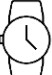
\includegraphics[height=1.00cm]{images/app_cronometro_1}} \newline \textbf{Opzione 2) }ciotolina con cucchiaino \newline \raisebox{-0.2\height}{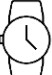
\includegraphics[height=1.00cm]{images/app_cronometro_1}} & \textbf{\emph{``Adesso disegniamo insieme. Ascoltami attentamente perché alcune volte ti dirò di andare LENTO-LENTO come una tartaruga }}\emph{(integrando con gesto e rallentando l'eloquio), }\textbf{\emph{così, guarda }}\emph{(mostrando), }\textbf{\emph{mentre altre dovrai andare VELOCE-VELOCE}}\textbf{, come una lepre} \emph{(sempre mostrando), }\textbf{\emph{così!}}\emph{''} \newline \textbf{\emph{``Ecco, adesso lo fai tutto da solo. Inizia a disegnare!''}} \newline \textbf{Step 1:} Trascorsi 5 secondi da quando ha iniziato a disegnare, dire (rallentando l'eloquio): \textbf{\emph{``Ora disegna LENTO-LENTO!''.}} \newline \textbf{Step 2: }dopo altri 5 secondi dire: \textbf{\emph{``Adesso disegna VELOCE- VELOCE!''}} \newline \textbf{Step 3: }dopo altri 5 secondi dire: \textbf{\emph{``Adesso disegna di nuovo LENTO-LENTO''}} & \textbf{\emph{2}}: modula autonomamente la velocità in base alle consegne e la mantiene fino al step successivo. \newline \textbf{\emph{1}}: modula la velocità ma non la mantiene fino allo step successivo dell'operatore (si interrompe prima) o riesce solo in alcuni comandi e non in altri. \newline \textbf{\emph{0}}: la velocità non varia o varia indipendentemente dalle istruzioni, senza intenzionalità o controllo & \textbf{   2} \newline \textbf{1} \newline \textbf{0} \\
   &  & \textbf{\emph{``Adesso cuciniamo l'impasto per la torta. Ascoltami attentamente perché alcune volte ti dirò di girare LENTO-LENTO}} (integrando con gesto e rallentando l'eloquio): \textbf{\emph{così, guarda}} (mostrando), \textbf{\emph{mentre altre dovrai girare VELOCE-VELOCE, così!}} (sempre mostrando)\textbf{''.} \newline \textbf{\emph{``Ecco, adesso lo fai tutto da solo. Inizia a girare!''}} \newline \textbf{Step 1: }Trascorsi 5 secondi da quando ha iniziato a girare dire (rallentando l'eloquio): \textbf{\emph{``Ora gira LENTO-LENTO!''.}} \newline \textbf{Step 2: }dopo altri 5 secondi dire: \textbf{\emph{``Adesso gira l'impasto VELOCE-VELOCE!''}} \newline \textbf{Step 3: }dopo altri 5 secondi dire: \textbf{\emph{``Adesso gira di nuovo LENTO- LENTO!''}} &  &  \\
  \multicolumn{5}{|p{20.64cm}|}{\textbf{NOTE:}} \\
\bottomrule
\end{tabular}
}}

\clearpage
\noindent\centerline{%
\rotatebox{90}{%
\footnotesize
\setlength{\tabcolsep}{3pt}
\begin{tabular}{|p{3.2cm}|p{2.8cm}|p{7.8cm}|p{5.0cm}|p{1.0cm}|}
\toprule
  \textbf{ITEM E DOMINIO} & \textbf{MATERIALE} & \textbf{ISTRUZIONI} & \multicolumn{2}{|p{6.21cm}|}{\textbf{PUNTEGGIO}} \\
\midrule
  \textbf{10.GIOCO DELLA STATUA } \newline \textbf{Dominio: }inibizione motoria & \raisebox{-0.2\height}{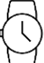
\includegraphics[height=1.00cm]{images/app_cronometro_2}}2 peluches & \textbf{Training} (non incide sul punteggio): Far familiarizzare il b con musica-pausa dicendo: \textbf{\emph{``Senti a volte c'è la musica e a volte non c'è più!''}}\textbf{.  }Poi fare un breve training insieme a b e dire: \textbf{\emph{``gli orsetti ballano quando c'è la musica, e dormono quando la musica non c'è'' }}(far vedere i pupazzi che ballano e si fermano). \newline \textbf{\emph{``Ora prova anche tu''}} passare un pupazzo al b e farlo insieme. \newline \textbf{Fase test:} \textbf{\emph{``Adesso continua tu, ricorda che, l'orsetto balla solo quando c'è la musica, altrimenti dorme!'' }} \newline Proporre---> 10s musica- 10s stop; 10s musica; 10s stop. \newline \textbf{Fase interferenza }\textbf{\emph{OPZIONALE }}(\uline{solo se superata la prima parte}, almeno 1): \newline Dire: \textbf{\emph{``Adesso lo rifacciamo, ma io non sono tanto brava, non mi riesco a fermare... l'orsetto balla solo quando c'è la musica, e dorme quando la musica non c'è''}}\emph{, }nel mentre fornire al b un modello di ciò che dovrà fare utilizzando i due orsetti in mani differenti. \newline Poi dire: \textbf{\emph{``Adesso continua tu, ricorda che, l'orsetto balla solo quando c'è la musica, e dorme quando la musica non c'è!''.}} Nel mentre che il b procede, muovere l'orsetto non rispettando la consegna. & \textbf{\emph{2}}: b ferma il pupazzo ad entrambi gli stop \newline \textbf{*}ammessi piccoli movimenti. \newline \textbf{\emph{1}}: b resiste per metà del tempo o ferma il pupazzo in solo uno dei 2 stop. \newline \textbf{\emph{0}}: b non rispetta le consegne, non si ferma allo stop della musica o si ferma per tempi molto ridotti \newline \textbf{NV: }b non muove i pupazzi \newline \textbf{Stella:} se il bambino supera anche la parte opzionale & \textbf{2} \newline \textbf{1} \newline \textbf{   0} \newline \textbf{NV} \newline \raisebox{-0.2\height}{
\includegraphics[height=0.68cm]{images/app_stella}} \\
  \multicolumn{5}{|p{20.64cm}|}{\textbf{NOTE: }ANNOTARE SE IL BAMBINO NON MUOVE I PUPAZZI (``NON VALUTABILE'')} \\
\bottomrule
\end{tabular}
}}

\clearpage
\noindent\centerline{%
\rotatebox{90}{%
\footnotesize
\setlength{\tabcolsep}{3pt}
\begin{tabular}{|p{3.2cm}|p{2.8cm}|p{7.8cm}|p{5.0cm}|p{1.0cm}|}
\toprule
  \textbf{ITEM E DOMINIO} & \textbf{MATERIALE} & \textbf{ISTRUZIONI} & \multicolumn{2}{|p{6.21cm}|}{\textbf{PUNTEGGIO}} \\
\midrule
  \textbf{11.SPARABOLLE} \newline \textbf{Dominio: }delyed gratification & Sparabolle \newline \raisebox{-0.2\height}{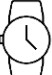
\includegraphics[height=1.00cm]{images/app_cronometro_1}} & \textbf{\emph{``Guarda, questo sparabolle!!''}} (o \textbf{``guarda questo panda, può sparare bolle!!''}). Mostrare il funzionamento accendendo e spegnendo le bolle e dopo una breve esplorazione dire: \textbf{\emph{``Lo sparabolle }}\textbf{(}o\textbf{ ``il panda'')}\textbf{\emph{ si è stancato, deve riposarsi!}} \textbf{\emph{Aspettiamo insieme prima che inizi a fare le bolle. Aspetta mi raccomando, lo sparabolle }}\textbf{(}o\textbf{ ``il panda'')}\textbf{\emph{ è veramente molto stanco! Più aspettiamo più bolle farà dopo!''}} \newline Mettere lo sparabolle sul tavolo in posizione raggiungibile al bambino e \textbf{\uline{cronometrare}} da questo momento. \newline Dopo circa 20 sec riattivare lo sparabolle (il panda). & \textbf{\emph{2}}: b aspetta 20 sec prima di attivare/toccare lo sparabolle \newline \textbf{1: }b aspetta 10 sec prima di attivare/toccare lo sparabolle \newline \textbf{\emph{0}}: b non attende (perde interesse, lo tocca, protesta ecc) \newline \textbf{\emph{NV}}: il b non è interessato & \textbf{2} \newline \textbf{1} \newline \textbf{0} \newline \textbf{NV} \\
   &  &  &  &  \\
   &  &  &  &  \\
  \multicolumn{5}{|p{20.64cm}|}{\textbf{NOTE: }ANNOTARE SE IL BAMBINO NON È INTERESSATO (``NON VALUTABILE'')} \\
\bottomrule
\end{tabular}
}}

\clearpage
\noindent\centerline{%
\rotatebox{90}{%
\footnotesize
\setlength{\tabcolsep}{3pt}
\begin{tabular}{|p{3.2cm}|p{2.8cm}|p{7.8cm}|p{5.0cm}|p{1.0cm}|}
\toprule
  \textbf{ITEM E DOMINIO} & \textbf{MATERIALI} & \textbf{ISTRUZIONI} & \multicolumn{2}{|p{6.21cm}|}{\textbf{PUNTEGGIO}} \\
\midrule
  \textbf{12.ASTA CON ANELLI} \newline \textbf{Dominio:} \newline pianificazione & Asta con anelli (5 aperti e 2 chiusi) & Mostrare il modello ordinato e poi dire: \textbf{\emph{``Lui è Pinco Pallo. Adesso gli facciamo uno scherzo… }}\emph{Disfare il modello e disporre l'asta e gli anelli aperti e chiusi davanti a b e dire:}\textbf{\emph{ Adesso va ricostruito! Fai attenzione e cerca di ricostruirlo più veloce puoi!''}} & \textbf{\emph{2}}: b inserisce tutti gli anelli con il foro, escludendo quelli senza foro \newline \textbf{\emph{1}}: b procede per tentativi ed errori tenta di inserire un anello chiuso nell'asta e poi procede \newline \textbf{\emph{0}}: b prova a inserire entrambi gli anelli chiusi nell'asta, perseverando. \newline \textbf{Stella: }b inserisce gli anelli nell'asta seguendo un criterio di grandezza & \textbf{2} \newline \textbf{1} \newline \textbf{0} \newline \raisebox{-0.2\height}{
\includegraphics[height=0.68cm]{images/app_stella}} \\
  \multicolumn{5}{|p{20.64cm}|}{\textbf{NOTE: }} \\
\bottomrule
\end{tabular}
}}

\clearpage
\noindent\centerline{%
\rotatebox{90}{%
\footnotesize
\setlength{\tabcolsep}{3pt}
\begin{tabular}{|p{3.2cm}|p{2.8cm}|p{7.8cm}|p{5.0cm}|p{1.0cm}|}
\toprule
  \textbf{ITEM E DOMINIO} & \textbf{MATERIALE} & \textbf{ISTRUZIONI} & \multicolumn{2}{|p{6.21cm}|}{\textbf{PUNTEGGIO}} \\
\midrule
  \textbf{13. TORTE} \newline \textbf{Dominio: }classificazione + flessibilità & 2 torte + frutta: mele, pere e banane GRANDI in 3 diversi colori (rosso- giallo- verde) \newline \raisebox{-0.2\height}{
\includegraphics[height=1.00cm]{images/app_stop_1}} & Disporre in maniera causale gli ingredienti davanti al bambino, lasciarlo esplorare e dire:\textbf{ ``ecco degli ingredienti per fare una torta, guarda abbiamo: mele, pere e banane''. }Lasciarlo esplorare e familiarizzare con i frutti. \newline \textbf{FASE }\textbf{\uline{COLORE}}\textbf{:} mettere le due torte davanti al bambino e dire: \textbf{``Adesso prepariamo delle torte speciali, per esempio una torta la facciamo così, tutta rossa…''. }L'esaminatore mette 3 ingredienti rossi sulla torta e poi dice: \textbf{``Adesso continua tu, come puoi fare quest'altra torta?''}. Attendere che sia b a classificare gli ingredienti necessari per le altre torte (verdi o gialli). \newline \textbf{*}Se b non si organizza, l'esaminatore mette un unico ingrediente verde su un'altra torta e poi dice: \textbf{``Questa potremmo farla tutta verde. Adesso continua tu…'' }Disfare quest'ultima torta e poi dire: \textbf{``E quest'ultima torta come puoi farla?''} \newline \textbf{*}Se b dispone gli ingredienti in modo casuale, riproporre il modello rosso e dire: \textbf{``ricominciamo, guarda bene! Io faccio quella rossa e tu fai le altre''} \newline \textbf{FASE }\textbf{\uline{FORMA}}\textbf{ OPZIONALE: (}\textbf{\uline{solo se è stata superata la prima parte}}\textbf{)} \newline \textbf{``Adesso facciamo una torta ancora diversa con questi ingredienti. Per esempio una torta la facciamo così, tutta di mele… Adesso continua tu, come puoi fare quest'altra torta?'' }(banane o pere). Poi procedere come nella fase colore\textbf{*}. & \textbf{\emph{2}}: b realizza da solo le due torte, classificando per colore entrambe le volte, senza necessità di esempi \newline \textbf{\emph{1: }}dopo l'esempio dell'esaminatore (torta verde), b fa almeno 1 torta diversa applicando il criterio colore. \newline \textbf{0: }b non realizza torte in base al colore. \newline \textbf{Stella: }supera anche la parte opzionale \textbf{``forma''} & \textbf{2} \newline \textbf{1} \newline \textbf{0} \newline \raisebox{-0.2\height}{
\includegraphics[height=0.68cm]{images/app_stella}} \\
  \multicolumn{5}{|p{20.64cm}|}{\textbf{NOTE:}} \\
\bottomrule
\end{tabular}
}}

\clearpage
\noindent\centerline{%
\rotatebox{90}{%
\footnotesize
\setlength{\tabcolsep}{3pt}
\begin{tabular}{|p{3.2cm}|p{2.8cm}|p{7.8cm}|p{5.0cm}|p{1.0cm}|}
\toprule
  \textbf{ITEM E DOMINIO} & \textbf{MATERIALE} & \textbf{ISTRUZIONI} & \multicolumn{2}{|p{6.21cm}|}{\textbf{PUNTEGGIO}} \\
\midrule
  \textbf{14.TORTA NEL FORNO Dominio: }inibizione motoria & Torta + forno \newline \raisebox{-0.2\height}{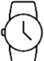
\includegraphics[height=1.00cm]{images/app_cronometro_3}} & Far scegliere al bambino una delle torte precedentemente preparata e dire: \textbf{\emph{``Adesso mettiamo la torta in forno e aspettiamo che sia cotta. Quando è pronta suonerà il campanello''.}} \newline Impostare timer di 1 min e cronometrare quanto passa prima che il bambino tocca il forno (ma attendere comunque la fine del minuto) poi dire: \textbf{``è suonato il timer, adesso possiamo prenderla''.} & \textbf{\emph{2}}: b attende fino al suono del timer (1 min), prima di toccare il forno \newline \textbf{\emph{1}}: b attende almeno 30 sec, prima di toccare il forno \newline \textbf{\emph{0}}: b non attende (perde interesse, lo tocca, protesta etc.) & \textbf{2} \newline \textbf{1} \newline \textbf{0} \\
  \multicolumn{5}{|p{20.64cm}|}{\textbf{NOTE:}} \\
\bottomrule
\end{tabular}
}}

\clearpage
\noindent\centerline{%
\rotatebox{90}{%
\footnotesize
\setlength{\tabcolsep}{3pt}
\begin{tabular}{|p{3.2cm}|p{2.8cm}|p{7.8cm}|p{5.0cm}|p{1.0cm}|}
\toprule
  \textbf{ITEM E DOMINIO} & \textbf{MATERIALE} & \textbf{ISTRUZIONI} & \multicolumn{2}{|p{6.21cm}|}{\textbf{PUNTEGGIO}} \\
\midrule
  \textbf{15.GIOCO LIBERO} & Kit del gioco libero & Posizionare i giochi di fronte a b e dire: \textbf{\emph{``Questi sono qua per te. Puoi giocarci}} \newline \textbf{\emph{come vuoi''.}} & \textbf{\emph{2}}: accetta e si adatta all'intervento dell'adulto integrando, imitando o modificando il suo schema \newline \textbf{\emph{1}}: accetta e imita ma con scarsa modifica del suo schema. \newline \textbf{0}: non accetta o ignora l'intervento dell'adulto, continuando a giocare autonomamente. & \textbf{2} \newline \textbf{1} \newline \textbf{0} \\
  \textbf{Dominio: }flessibilità & \raisebox{-0.2\height}{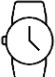
\includegraphics[height=1.00cm]{images/app_cronometro_4}} & Lasciare giocare autonomamente b. Se b non avvia il gioco in modo spontaneo, si può proporre un'attività partendo da materiali d'interesse. &  &  \\
   &  & \textbf{Intervento: } \newline Durante il gioco, dopo almeno 3 min, provare ad inserirsi variando o arricchendo il gioco del b. &  &  \\
  \multicolumn{5}{|p{20.64cm}|}{\textbf{NOTE:}} \\
\bottomrule
\end{tabular}
}}

\clearpage

\section*{Legenda}

\textbf{\emph{   LEGENDA:}}

: \textbf{SALTARE ITEM} \textbf{(}\textbf{\uline{SOMMINISTRARE ITEM 3 SOLO SE IL BAMBINO       RAGGIUNGE UN PUNTEGGIO DI 1/2 NELL'ITEM 2}}\textbf{)}\raisebox{-0.2\height}{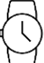
\includegraphics[height=1.00cm]{images/app_cronometro_2}}\textbf{:} \textbf{CRONOMETRARE                                                                                                             }\raisebox{-0.2\height}{
\includegraphics[height=1.00cm]{images/app_item_opzionale}}

\raisebox{-0.2\height}{
\includegraphics[height=1.00cm]{images/app_stop_2}}

\textbf{: STOP (non continuare con la seconda parte dell'item)}

\raisebox{-0.2\height}{
\includegraphics[height=1.00cm]{images/app_stella}}: \textbf{da} \textbf{barrare quando vengono superate anche richieste supplementari, che non incidono sul punteggio.}
